\documentclass{article}
\usepackage[utf8]{inputenc} % Så vi kan rocka på värmländska 
\usepackage[parfill]{parskip}  %För att slippa den där jävla indenteringen
\usepackage{graphicx} % För plottarna
\usepackage{color}  %plottarna

\title{Player positions in the NBA \\
using unsupervised learning \\ 
\large  732A61 Clustering and Association Analysis }
\author{Emil Klasson Svensson }
\date{Linköping University \\
June 2017}

\begin{document}

\maketitle

\newpage

\section{Introduction}

Basketball is one of the largest and most popular sports in the world (citation, wiki).  It is a team sport where two teams fielding five player each trying to put the the ball trough the opponents basket with the team scoring most points being the winning side. One team usualy fields different types players accorind to their given position, this is a position given arbitrary given the players pysical apperance.  The goal is to find new positions clustering algorithms given data rather than the tratidional approach. The project will focus on analysing data collected from the National Basket Association (NBA) which is today regarded as the leauge with has the highest level of professional basketball.

This project is  loosely based around a article written by Dwight Lutz called  ”A Cluster Analysis of NBA Players” which revolves around finding clusters of NBA-players (basketball players) and giving them a new class-labeled for basketball players positions on court.
 

%\subsection{What is Basketball?}


\subsection{Positions in Basketball}

Traditionally players are labeled according to the respective task on the court, called positions. In this standard there are five different positions

\begin{enumerate}
\item Center 
\item Power Forward
\item Small Forward
\item Shooting Guard
\item Point Guard
\end{enumerate}

Small and fast players are often referred to as guards (point guard/shooting guard) with main focus on handeling, distributing and scoring. Tall and strong players are labeled (power/small-) forward or center. The small forward task i mainly scoring and grabbing rebounds while Power forward and Center have a bigger role in setting screens for smaller players and grabbing rebounds,   There is no formal way of determining what position a player should be according to these five current positions and it is up to coaches to decide this and this affects the way the player on the position play and acts. 

In the modern NBA something that is called ”positionless basketball” have gained popularity with many coaches moving away from defining their players according to the classic positions and playing different line ups with players wich traditionally would play on the same position. (citation?) This trend has led to journalists inventing more lables to describe players in order to find some structure. 

\subsection{Objective}

The goal with this project will be to via multivariate cluster analysis identify new and  more appropriate labels for players defined by their performance on the court rather then traditional preceptions. A qualative and quantative analysis of the clusters and members of the different clusters will be done to evaluate and discuss the quality of the result.  



\section{Variables}

The data collected are from NBAs own repository avaliable att nba.com using webscraping tools and some processing. The set in total contains 34 different variables from 271 players during the season of 2015-2016 where all variables were aggregated by average per game. Players playing under 40 games were excluded from the data set since only frequently used player are of interested to cluster.  The decision to only use data from one year instead of over consecutive years was determined by the goal of the project. Seeing how the trend of so called possitionless basketball is a relatively new fenonema having data spanning over multiple years might wash away characteristics of averages for players that have been in the leauge during multiple years. The down side of this is the problem of having to few observations may lead to clusters beeing hard to define since a lower amout of observations. In the table below all variables used in the clustering are presented. 

\begin{table}[ht]
\centering
\begin{tabular}{rll}
  \hline
 & \textbf{Abbrivations} & \textbf{Explanation} \\ 
  \hline
1 & MIN & Minutes played \\ 
  2 & FGA & Field Goals Attempted \\ 
  3 & FG\_PCT & Field Goal Percentage \\ 
  4 & FG3A & 3-Point Field Goals Attempted \\ 
  5 & FG3\_PCT & 3-Point Field Goal Percentage \\ 
  6 & FTA & Free Throws Attempted \\ 
  7 & FT\_PCT & Free Throw Percentage \\ 
  8 & OREB & Offensive rebound \\ 
  9 & DREB & Defensive Rebound \\ 
  10 & AST & Assist \\ 
  11 & STL & Steals \\ 
  12 & BLK & Blocks \\ 
  13 & TOV & Turnovers \\ 
  14 & PTS & Points Made \\ 
  15 & Dist..Feet & Distance in feet \\ 
  16 & AvgSpeed & Average Speed \\
   \hline
\end{tabular}
\caption{\textit{Variables used in clustering and visualisation}} 
\end{table}

In the original collected dataset each player had 31 different variables (excluding player names and player ID) avaliable in Appendix A . All of these variables are aggregated as the average of games played.   Many of the original variables are naturally connected and correlated as for example Field Goal - Percentage (FG\_PCT) is a function of the variables Field Goals Made, Field Goals Attempted. So in order to try to reduce the number of dimensions in the dataset but still keep information variables that describes Made - Fields Goals, 3 Point Field Goals and Free Throws were removed since they are described in their respective percentages, altough this is true for the number of attempts it is an interessting variable since that players taking shots indicates some sort of action on court compared to the act of making a shot which is just one of two consequenses of shooting the ball.  The variable EFF was also removed since it is a function of several of the other variables and doesn't describe any action on the court. Other than that all variables removed were removed because they are a superset or subset of each other.

 All variables were standardized before clustering in the following manner to reduce the number of 
 $$z_{ij} = \frac{x_{ij} - \mu_{j}}{\sigma_{j}}$$ 

%Nagat skrap eller mening som kanske ar bra senare.
%Since this project aims to identify and find different types of players as many defining characteristics were preferred as well defined 

\newpage


\section{Method}

\subsection{t-SNE}


t distributed Stochastic Neighbourhood Embedding (t-SNE) is a dimensionality reduction technique that aim to take a data set with k dimension and project them on to a 2 dimensional or 3 dimensional plane with the goal to display similar objects from the high dimensional data set close to each other in the lower dimensional plane. 

It uses conditional probabilities $p_i|j$ to model the high dimensional probability of observation xi picking xj as its neighbour under a t-distibuted kernel. This is then compared to the probability $q_i|j$  which is is the same but in the low dimensional space where it tries to project these observations. These distributions are then compared with the Kullback Leibler (RATT NAMN???) divergence, this is the algorithms cost function where the high and low dimensions match with the same probability reaches its minimum. 

$$C = KL(P||Q)=\sum_i\sum_jp_{ij}log(\frac{p_{ij}}{q_{ij}})$$

The minimization technique used is gradient decent which iteratively walks through the space in order to find a local minimum with a selected step size in proportion to the second derivative of the cost function also known as the gradient.

The variance in the kernels are set by the parameter perplexity which i a tunable hyper parameter that tries to catch the relationship between the local and the global structure of the data in order to preserve it in the low dimensional space. According to the authors of the paper the algorithm provides stable results for values between 5 and 50, in this project different perplexity valuest will be explored and evaluated. 

The implementation used is implemented in R and is from the package "tsne". 

Lite mer formler 
Kanske pladdra lite mer, men det kanske ar nog.


\subsection{EM-algorithm}

Expectation–maximization algorithm  (EM Algorithm) is a technique that uses the observed data and a latent variable that is the unobserved data and tries to find the maximum likelihood estimation (MLE). It is a general method with many applications in the area of data mining where clustering is one of them.

In this project a mixature of gaussians will be used due to the fact that it is the only avaliable implementation in R . The package name is mclust. This leads to an assumption that all observations are independently identicaly normal distributed. This assumption is in this project questionable since there every player on court impacts eachother in significat way.  But previous result has show that the normality assumption is farily robust and are therefor accepted. 

All of the observed data points are denoted X and the unobserved (Also called latent variables) points are denoted Z. These two variables are assumed to each have some sort of probability distribution given a unkown parameter $\theta$. In the case of clustering the cluster-group is considerd to be unkown and is denoted as the latent variable in this case.  Combining these two distributions will give us our joint distribution. From here the algorithm starts itterating through the two steps, the Expectation-step and the second one beeing the maximization - step.


In the E-step we calculate the probability for each observation in Z belonging too the different cluster lables given the data and a current estimate of this parameter theta that we are updating.

$$\gamma(z_{nk}) = \frac{\pi_k N(x_n|\mathbf{\mu}_k,\mathbf{\Sigma}_k)} {\sum_{j=1}^{K}  \pi_jN(x_n|\mathbf{\mu}_j,\mathbf{\Sigma}_j)}$$

With this information we then move on to the M-step where the probabillities from the E-step are used to compute the weighted averages between the probabillities for $Z_ij$ belonging to each cluster multiplied with the obser value $X_ij$ to get the cluster centroids. 

$$\mathbf{\mu}_k^{new} = \frac{1}{N_k} \sum_{n=1}^N\gamma(z_{nk})x_n$$

$$\mathbf{\Sigma}_k^{new} = \frac{1}{N_k} \sum_{n=1}^N\gamma(z_{nk})(x_n-\mathbf{\mu}_k^{new})(x_n-\mathbf{\mu}_k^{new})^T$$

$$ \pi_k^{new}= \frac{N_k}{N} $$ 
where
$$  N_k = \sum_{n=1}^N \gamma(z_{nk})$$

With the new parameters we evaluate the the log of likelihood with these newly updated parameter and check if we have found a stable result, if not, these two steps are  repeated back and forth untill an stable is found or the max number of itterations is reached. Since the joint likelihood function is almost always multimodal the algorithm is only guaranteed to find a local optimum. 

This uppdating procedurec means that the observations are not hard-assigned to one cluster untill convergence (via argmax) but instead given a probability to be in each cluster allowing for more dynamical clustering approach to the data in the way that it is able to find different density regions in the data. 

Kanske lite om relationen till K-means för att runda upp det hela? 


With these two parameters we define a joint distribution that we then try to find the maximum likelihood estimated parameters via a expectation and a maximization step.

\newpage

\section{Results}

\subsection{Visualization with t-SNE}

The process of finding a good visualization for t-SNE for this project started out with a sequence of 5 different values from 10 to 50 to try to get a feeling for how the algorithm handled the data. On all levels of perplexity the algorithm seemed to to not any noticeable changes in minimizing the costfunction after around 1500 itterations. For the perplexity number the lower values of perplexity seems to yield better separation between visually identified clusters. The projections placement in relationship to eachother were often time close to each other independent of the perplexity setting. Of the five initial runns values a perplexity of 10 was determined to be the best and values 5 and 15 for perplexity were explored to try to se the generall trend of how the projections behaved. When trying a perplexity above 10 the separation seemed to be washing away a bit. For values in the lower range with a perplexity of 5 the separation seems to be increasing and was chosen as the final . 

\begin{figure}[h]
 \centering
 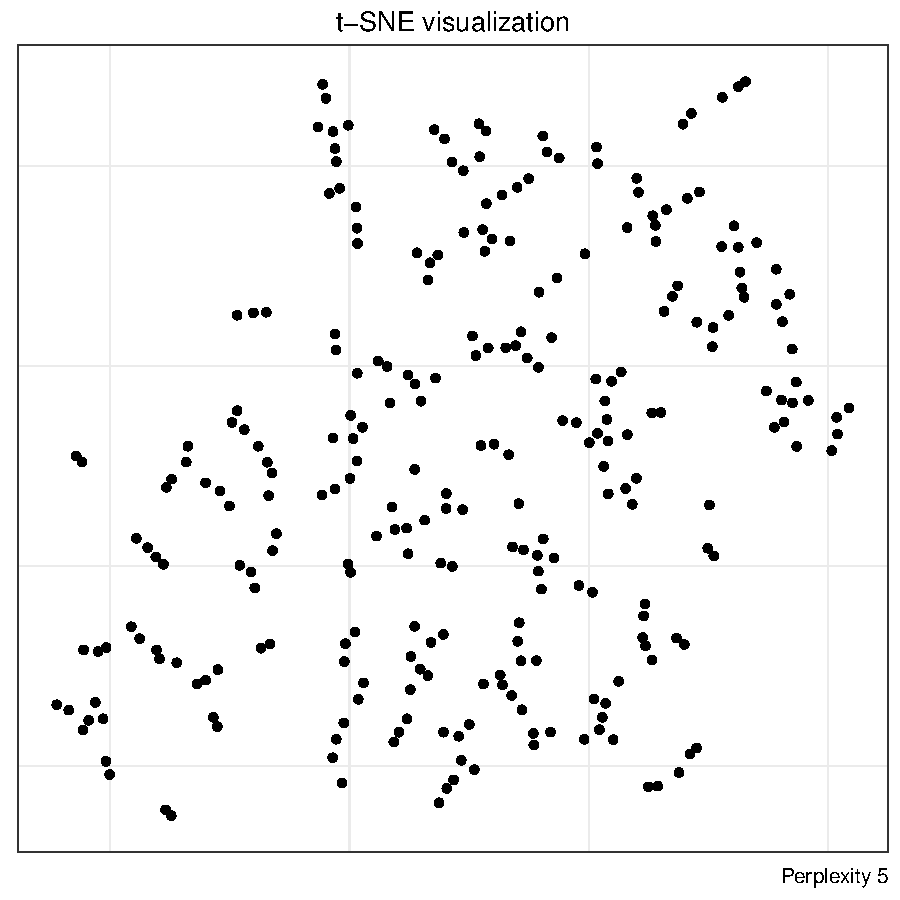
\includegraphics[height=10cm]{tsneper5}.
 \caption{t-SNE visualization with perplexity 5}
 \label{figure:1}
\end{figure}

In the lower left corner there seem to be one or two clusters with in total around 20 similar observations.  Above this cluster there seem to be a similar sized cluster. In the bottom middle there also seem to be a cluster that could be divided in to several small clusters. The same goes for what seems to be a cluster in the middle of the graph. In the right side of the graph there seem to be one cluster moving up towards the corner where another cluster appears. Around these two clusters are two "strings" with players that are not a part of the clusters one in the middle top and one in the top right corner.

 
\begin{figure}[h]
 \centering
 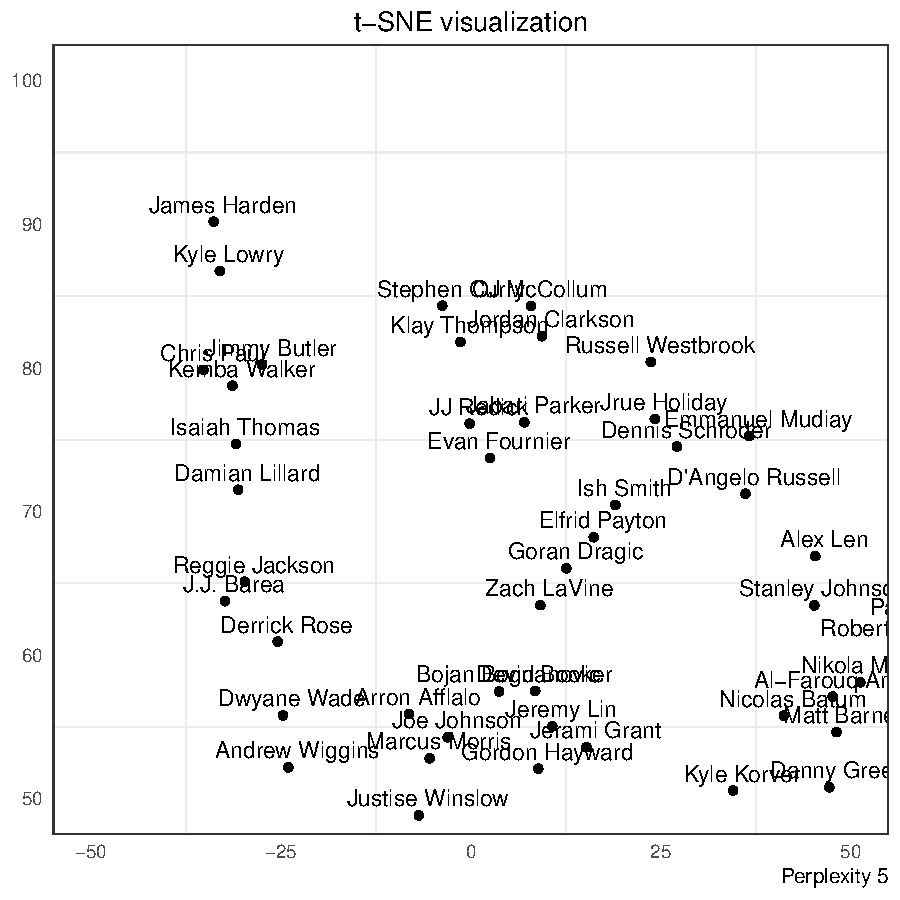
\includegraphics[height=10cm]{zoom1}.
 \caption{t-SNE visualization with perplexity 5 zoomed in}
 \label{figure:1}
\end{figure}

 

\section{Discussion}

It would be interesting in a larger project to compare clustering over different seasons and compare them to the original positions.

Deciding between 5-10 the improvments were tought because what could be improvments could as likely be assigned as random.
 This indicates that the algorithm manages to capture some of the local structure of the data regardless of the perplexity. 

\end{document}

\section{Appendix}
\subsection{Appendix A}



